% This is part of Un soupçon de mathématique sans être agressif pour autant
% Copyright (c) 2013
%   Laurent Claessens
% See the file fdl-1.3.txt for copying conditions.


\documentclass{beamer}

\usepackage[utf8]{inputenc}
\usepackage[T1]{fontenc}

\usepackage{textcomp}
\usepackage{lmodern}
\usepackage[english,frenchb]{babel}

\usepackage{calc}   % Les dépendances de phystricks si on n'utilise que le pdf.
\usepackage[cdot,thinqspace,amssymb]{SIunits} 
\usepackage{multicol}
\usepackage{wrapfig}
\usepackage{framed}
% Ce bout de code provient de BrunoJ
% https://brunoj.wordpress.com/2009/10/08/latex-the-framed-minipage/
\newsavebox{\fmbox}
 \newenvironment{fmpage}[1]
 {\begin{lrbox}{\fmbox}\begin{minipage}{#1}}
     {\end{minipage}\end{lrbox}
     \fbox{\usebox{\fmbox}}
 }
\newcommand{\vect}[1]{\overrightarrow{#1}}    % Cette macro est codée en dur dans phystricksDefVecteurAXDDGP et dans d'autres

\newcommand{\mC}{\mathcal{C}}

\usetheme{default}
\begin{document}

% Le 9 n'a pas encore été fait en classe
\begin{frame}{Calcul mental 11}
    \begin{enumerate}
        \item
            Soit la fonction \( f(x)=3x^2-7\) et \( \mC\) la courbe représentative de \( f\).
            \begin{itemize}
                \item Donner les coordonnées d'un point de \( \mC\)
                \item Donner les coordonnées d'un point d'abscisse \( 3\) sur \( \mC\).
                \item Donner les coordonnées d'un point d'ordonnée \( 5\) sur \( \mC\).
            \end{itemize}
    \end{enumerate}
\end{frame}

\begin{frame}{Calcul mental 10}

    \pause

    \begin{enumerate}

        \item
            Calculer
            \begin{equation}
                52\times 3+12\times 3.
            \end{equation}
            \pause

        \item


        \begin{itemize}
            \item Si \( AB=3\), que vaut \( AC\) ?
            \item Même question si \( AB=x\).
        \end{itemize}
            \begin{center}
            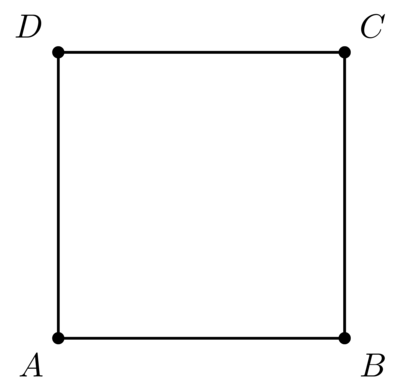
\includegraphics[width=3.5cm]{Picture_FIGLabelFigGUEjmmRPICTGUEjmmR-for_eps.png}
            \end{center}

    \item
        \pause
        \begin{itemize}
            \item 
    Développer et réduire $(x+1)(x-1)$, 
\item
    Factoriser $x^2-1$.
        \end{itemize}
    \end{enumerate}
\end{frame}

\begin{frame}{Calcul mental 9}

    \pause
    \begin{enumerate}
        \item
            QCM (une seule réponse correcte). Soient \( A(2;-1)\) et \( B(-1;-1)\). La droite \( (AB)\) \ldots
            \begin{enumerate}
                \item
                    a pour équation \( x=-1\)
                \item
                    a pour équation \( y=-1\)
                \item
                    n'a pas de coefficient directeur.
            \end{enumerate}

            \pause
        \item
            Calculer 
            \begin{equation*}
                1- \frac{1}{ 3 }
            \end{equation*}
            \pause
        \item
            Calculer 
            \begin{equation*}
                1- \frac{1}{ a }
            \end{equation*}
            \pause
        \item
            Dire si \( x=5\) est solution de l'inéquation
            \begin{equation}
                \frac{ 6 }{ x }<3
            \end{equation}
            
    \end{enumerate}
\end{frame}

\begin{frame}{Calcul mental 8}
    \begin{enumerate}
            \pause
        \item

                Dans le repère suivant, \( \vect{ AB }\) a pour coordonnées 
            \begin{tabular}[]{cccc}

                \begin{minipage}{0.3\textwidth}
                \begin{center}
        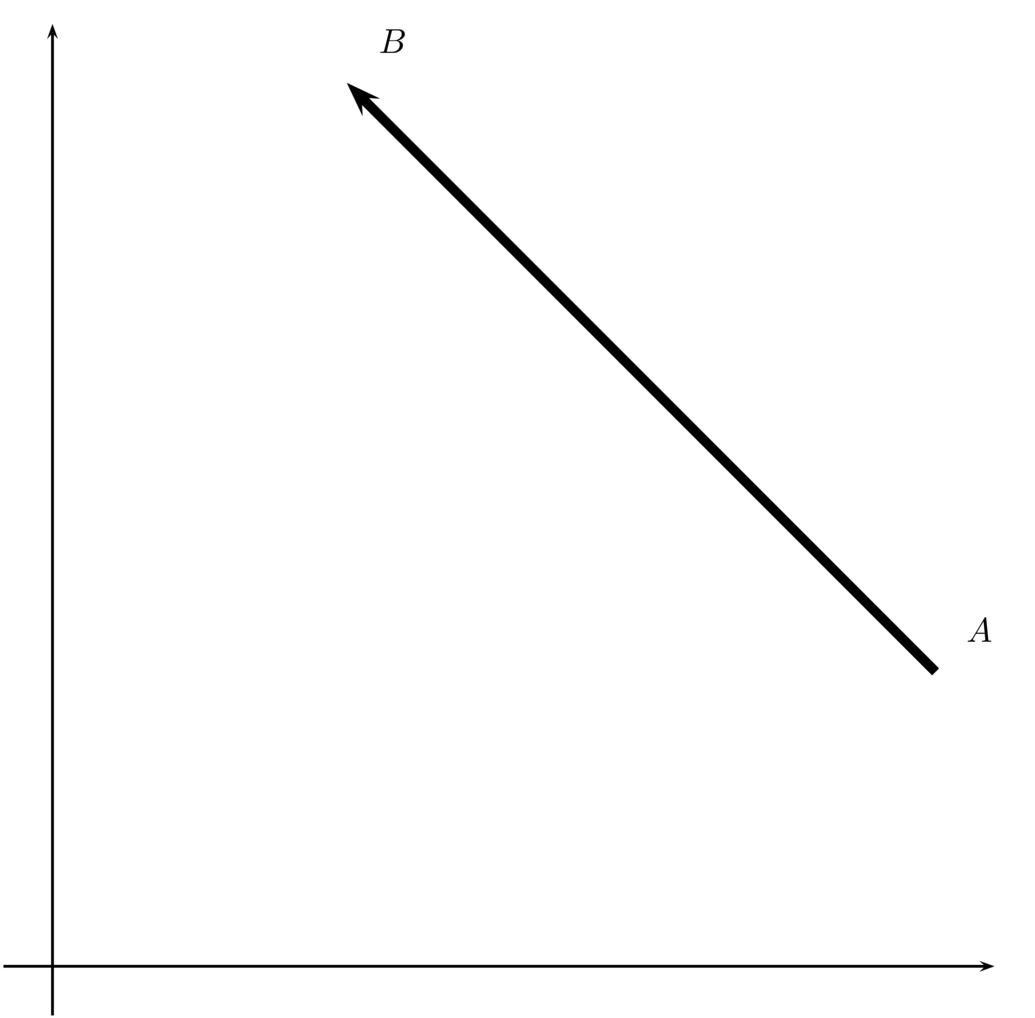
\includegraphics[width=2.6cm]{Picture_FIGLabelFigUZlaYZPICTUZlaYZ-for_eps.png}
                \end{center}
                \end{minipage}
                
   &\( \begin{pmatrix}
       -3 \\ 
       -8 
   \end{pmatrix}\)&\( \begin{pmatrix}
       -3 \\ 
       8 
   \end{pmatrix}\)&\( \begin{pmatrix}
       3 \\ 
       -8 
   \end{pmatrix}\)\\
            \end{tabular}
            
 \pause            
        \item

            Si \( A\) est le point de coordonnées \( (3;-1)\) et \( X\) celui de coordonnées \( (7;-4)\), quelles sont les coordonnées de \( \vect{ AX }\) ?

            \pause
\item

    Calculer
    \begin{equation}
        \frac{ 12\times 50+5 }{ 5 }
    \end{equation}

    \pause

\item

    Pour quel \( y\) le point \( (4;y)\) est-il sur le graphe de la fonction \( f(x)=3x-2\) ?

    \end{enumerate}
    
\end{frame}

\begin{frame}{Calcul mental 7}
    \begin{enumerate}
            \pause
        \item
            Résoudre \( -3x+7=-8\)
        \item
            \pause
            Quel est le signe de \( (x-3)(x+4)\) lorsque \( x=-10\) ?
        \item
            \pause
            Donner un encadrement de \( f(5)\).
    \begin{equation*}
        \begin{array}[]{|c||ccccccccc|}
            \hline
            x&-10&&-3&&4&&6&&10\\
            \hline\hline
            &&&0&&&&2&&\\
            f(x)&&\nearrow&&\searrow&&\nearrow&&\searrow&\\
            &1&&&&-12&&&&2\\
            \hline
        \end{array}
    \end{equation*}
        \item
            \pause
                Qu'affiche le programme suivant ?
\begin{fmpage}{0.9\linewidth}

    $S = 0$

    Pour \( i\) allant de \( 1\) à \( 4\) :

    \hspace{1cm} \( S=S+i\)

    Afficher \( S\)

\end{fmpage}
    \end{enumerate}
\end{frame}

\begin{frame}{Calcul mental 6}
    \begin{enumerate}
        \item
            \pause
            Résoudre \( \frac{1}{ x }=4\)
        \item
            \pause
            Simplifier
            \begin{equation*}
                \frac{ x+2 }{ (x+2)(x-3) }.
            \end{equation*}
        \item
            \pause
            Qu'affiche l'algorithme suivant si on entre la valeur \( 4\) ?

\begin{fmpage}{0.9\linewidth}

    Demander \( x\)

    Si \( x < 2\) alors

    \hspace{1cm} \( P\) prend la valeur \( 2x-7 \)

    Si \( x >= 2 \) alors

    \hspace{1cm} \( P\) prend la valeur \( \frac{ 3 }{ 8 }x\)

    Afficher \( P\)

\end{fmpage}
        \item
            \pause
                Résoudre \( 2x+60=4\).

    \end{enumerate}
\end{frame}

\begin{frame}{Calcul mental 5}

    \begin{enumerate}
        \item

    \pause
            Écrire sous forme d'une somme : \( (x-4)^2\)

        \item
    \pause
            Simplifier :
            \begin{equation}
                \frac{ 4bx+b^2 }{ 2b }.
            \end{equation}
        \item

    \pause
            Résoudre : \( (x+2)(x-1)=0\).

        \item
    \pause
            Quelle est la longueur du segment joignant \( A(3;7)\) et \( B(4;10)\) ?
        \item
    \pause
            Si \( f(x)=x^2-2\), que vaut \( f(-1)\) ?
            
    \end{enumerate}
\end{frame}

    

\begin{frame}{Calcul mental 4}

    \begin{enumerate}
        \item

    \pause
            \begin{multicols}{2}

                La figure ci-contre est un cube. Quelle est la nature du triangle \( AHD\) ?

                \columnbreak

                \input{Fig_MUriGyU.pstricks}
            \end{multicols}

        \item
    \pause
            Écrire sous forme d'une somme : $(x+3)^2$.
        \item
            \pause
            L'aire d'un carré est de \unit{11}{\centi\meter\squared}. Quelle est la longueur exacte de son côté ?
        \item
            \pause
            Simplifier 
            \begin{equation}
                \frac{ 8ax+a^2 }{ 2a }.
            \end{equation}
            
    \end{enumerate}
\end{frame}


\begin{frame}{Calcul mental 3}
    \pause
    \begin{enumerate}
        \item
            Résoudre \( (x+1)(x-17)=0\)
            \pause
        \item
            Simplifier
            \begin{equation}
                \frac{ 4x+8a }{ 2 }.
            \end{equation}
            \pause
        \item
            Si \( f(x)=x^2-x\), que vaut \( f(4)\) ?
            \pause
        \item
            Quelle est la distance entre \( (0;4)\) et \( (2;-2)\) ?
            \pause
        \item
            La droite représentative de la fonction \( f(x)=3x+2\) est-elle parallèle à celle de \( g(x)=-3x+7\) ?
    \end{enumerate}
\end{frame}

\begin{frame}{Calcul mental 2}
    \pause
    \begin{enumerate}
        \item
            Simplifier \( \sqrt{72}\)
            \pause
        \item
            Calculer la distance entre \( (0;10)\) et \( (2;0)\).
            \pause
        \item
            Résoudre \( \frac{1}{ x }=\frac{ 2 }{ 3 }\).
            \pause
        \item
            Simplifier 
            \begin{equation*}
                \frac{ 12x+3b }{ 21 }.
            \end{equation*}
            \pause
        \item
            Calculer le milieu du segment entre \( (1;3)\) et \( (-3;8)\).
            \pause
        \item
            Résoudre
            \begin{equation*}
                (x+2)(x-1)=0.
            \end{equation*}
            \pause
    \end{enumerate}
    \begin{center}
        FIN pour aujourd'hui.
    \end{center}
\end{frame}

\begin{frame}{Calcul mental 1}

    \pause
    \begin{enumerate}
        \item
            Simplifier : \( \sqrt{12}\)

            \phantom{\( 2\sqrt{3}\)}

            \pause
        \item
            Les coordonnées du milieu entre \( (1;-2)\) et \( (6;4)\)
            \pause
        \item
            Simplifier 
            \begin{equation*}
                \frac{ 2xy }{ 4 }
            \end{equation*}
            \pause
        \item
            Simplifier
            \begin{equation*}
                \frac{ 8x+4a }{ 2 }
            \end{equation*}
            \pause
        \item
            Résoudre : \( 3x=12\).
            \pause
        \item
            Résoudre : \( 2x-6=4\).
    \end{enumerate}

\end{frame}

\end{document}
